\section{Automaten}
Ein System, das auf seine Eingänge reagiert und einen Ausgang produziert, der vom Eingangssignal und momentanen Zustand abhängt.\\
Bei synchronen Automaten besitzen alle Speicherelemente (FlipFlops) den gleichen Takteingang.

\subsection{Formale Beschreibung}
\begin{flushleft}
    \small
    \begin{tabular}{l p{33.5mm}}
        $X = (x_1, \dots, x_e)$ & Eingangsalphabet mit \emph{e} Eingängen\\
        $Y = (y_1, \dots, y_b)$ & Ausgangsalphabet mit \emph{b} Ausgängen\\
        $Z = (z_1, \dots, z_m)$ & Zustandsmenge mit \emph{m} internen Zuständen\\
        $Z_0 \in Z$ & Anfangszustand\\
        $f_{c1}:(X_n, Z_n) \rightarrow Z_{n+1}$ & Übergangsfunktion\\
        $f_{c2}:(X_n, Z_n) \rightarrow Y_n$ & Ausgangsfunktion
    \end{tabular}
\end{flushleft}
\subsection{Automatentypen}
% \subsubsection{Mealy}
% \begin{center}
%     \begin{minipage}{0.38\linewidth}
%         Ausgänge von inneren Zuständen \underline{und} Eingängen abhängig.
%         \begin{equation*}
%             Y_n = f_{c2}(X_n, Z_n)
%         \end{equation*}
%     \end{minipage}
%     \hfill
%     \begin{minipage}{0.6\linewidth}
%         \begin{center}
%             \begin{tikzpicture}[> = stealth, thick]
%                 \def\ulA{174};
%                 \def\mlA{180};
%                 \def\llA{186};
%                 \def\urA{6};
%                 \def\mrA{0};
%                 \def\lrA{-6};
%                 \node[draw, text width = 16.8mm] (outputFunc) {\small $f_{c2}:(X_n, Z_n)$};
%                 \node[draw, text width = 16.8mm, below = 2mm of outputFunc] (transFunc) {\small $f_{c1}:(X_n, Z_n)$};
%                 \node[draw = blue, fill = blue!20, text width = 16.8mm, below = 2mm of transFunc, align = center] (store) {\small Speicher};

%                 \node[left = 4mm of store.\llA] (clk) {\small CLK};
%                 \draw[->] (clk) -- (store.\llA);
                
%                 \path[draw, ->] (transFunc.\mrA) -- ($(transFunc.\mrA) + (0.2,0)$) -- ($(store.\mrA) + (0.2,0)$) node[midway, right] {$Z_{n+1}$} -- (store.\mrA);

%                 \path[draw, ->, blue] (store.\ulA) -- ($(store.\ulA) - (0.2,0)$) -- ($(transFunc.\llA) - (0.2,0)$) node[left, black] {$Z_n$} -- (transFunc.\llA); 
%                 \path[draw, ->, blue] ($(transFunc.\llA) - (0.2,0)$) -- ($(outputFunc.\llA) - (0.2,0)$) -- (outputFunc.\llA);

%                 \node[left = 4mm of outputFunc.\ulA] (input) {\small $X_n$};
%                 \path[draw, ->, red] (input) -- (outputFunc.\ulA);
%                 \path[draw, ->, red] (input) -- ($(input) + (0.4, 0)$) |- (transFunc.\ulA);

%                 \node[right = 4mm of outputFunc.\urA] (output) {\small $Y_n$};
%                 \draw[->] (outputFunc.\urA) -- (output);
%             \end{tikzpicture}
%         \end{center}
%     \end{minipage}
% \end{center}
% \subsubsection{Moore}
% \begin{center}
%     \begin{minipage}{0.38\linewidth}
%         Ausgänge nur von inneren Zuständen abhängig (keine Verbindung zwischen Input und Output).
%         \begin{equation*}
%             Y_n = f_{c2}(Z_n)
%         \end{equation*}
%     \end{minipage}
%     \hfill
%     \begin{minipage}{0.6\linewidth}
%         \begin{center}
%             \begin{tikzpicture}[> = stealth, thick]
%                 \def\ulA{174};
%                 \def\mlA{180};
%                 \def\llA{186};
%                 \def\urA{6};
%                 \def\mrA{0};
%                 \def\lrA{-6};
%                 \node[text width = 16.8mm, align = center, draw] (outputFunc) {\small $f_{c2}:(Z_n)$};
%                 \node[text width = 16.8mm, align = center, draw, below = 2mm of outputFunc] (transFunc) {\small $f_{c1}:(X_n, Z_n)$};
%                 \node[text width = 16.8mm, align = center, draw = blue, fill = blue!20, below = 2mm of transFunc] (store) {\small Speicher};

%                 \node[left = 4mm of store.\llA] (clk) {\small CLK};
%                 \draw[->] (clk) -- (store.\llA);
                
%                 \path[draw, ->] (transFunc.\mrA) -- ($(transFunc.\mrA) + (0.2,0)$) -- ($(store.\mrA) + (0.2,0)$) node[midway, right] {$Z_{n+1}$} -- (store.\mrA);

%                 \path[draw, ->, blue] (store.\ulA) -- ($(store.\ulA) - (0.2,0)$) -- ($(transFunc.\llA) - (0.2,0)$) node[midway, left, black] {$Z_n$} -- (transFunc.\llA); 
%                 \path[draw, ->, blue] ($(transFunc.\llA) - (0.2,0)$) -- ($(outputFunc.\llA) - (0.2,0)$) -- (outputFunc.\llA);

%                 \node[left = 4mm of transFunc.\ulA] (input) {\small $X_n$};
%                 \path[draw, ->, red] (input) -- (transFunc.\ulA);

%                 \node[right = 4mm of outputFunc.\urA] (output) {\small $Y_n$};
%                 \draw[->] (outputFunc.\urA) -- (output);
%             \end{tikzpicture}
%         \end{center}
%     \end{minipage}
% \end{center}
% \subsubsection{Medwedjew}
% \begin{center}
%     \begin{minipage}{0.38\linewidth}
%         Ausgänge entsprechen inneren Zuständen.
%         \begin{equation*}
%             Y_n = Z_n
%         \end{equation*}
%     \end{minipage}
%     \hfill
%     \begin{minipage}{0.6\linewidth}
%         \begin{center}
%             \begin{tikzpicture}[> = stealth, thick]
%                 \def\ulA{174};
%                 \def\mlA{180};
%                 \def\llA{186};
%                 \def\urA{6};
%                 \def\mrA{0};
%                 \def\lrA{-6};
%                 \node[text width = 16.8mm, align = center, draw, opacity = 0] (outputFunc) {\small $f_{c2}:(Z_n)$};
%                 \node[text width = 16.8mm, align = center, draw, below = 2mm of outputFunc] (transFunc) {\small $f_{c1}:(X_n, Z_n)$};
%                 \node[text width = 16.8mm, align = center, draw = blue, fill = blue!20, below = 2mm of transFunc] (store) {\small Speicher};
%                 \node[right = 4mm of outputFunc.\urA] (output) {\small $Y_n$};

%                 \node[left = 4mm of store.\llA] (clk) {\small CLK};
%                 \draw[->] (clk) -- (store.\llA);
                
%                 \path[draw, ->] (transFunc.\mrA) -- ($(transFunc.\mrA) + (0.2,0)$) -- ($(store.\mrA) + (0.2,0)$) node[midway, right] {$Z_{n+1}$} -- (store.\mrA);

%                 \path[draw, ->, blue] (store.\ulA) -- ($(store.\ulA) - (0.2,0)$) -- ($(transFunc.\llA) - (0.2,0)$) node[midway, left, black] {$Z_n$} -- (transFunc.\llA); 
%                 \path[draw, ->, blue] ($(transFunc.\llA) - (0.2,0)$) -- ($(outputFunc.\ulA) - (0.2,0)$) -- (output);

%                 \node[left = 4mm of transFunc.\ulA] (input) {\small $X_n$};
%                 \path[draw, ->, red] (input) -- (transFunc.\ulA);
%             \end{tikzpicture}
%         \end{center}
%     \end{minipage}
% \end{center}
\begin{flushleft}
    \renewcommand{\arraystretch}{1.25}
    \begin{tabular}{l p{44mm}}
        \textbf{Mealy} & Ausgänge von inneren Zuständen \underline{und} Eingängen abhängig\\
        & $Y_n = f_{c2}(X_n, Z_n)$\\
        \hline
        \textbf{Moore} & Ausgänge nur von inneren Zuständen abhängig (keine Verbindung zwischen Input und Output)\\
        & $Y_n = f_{c2}(Z_n)$\\
        \hline
        \textbf{Medwedjew} & Ausgänge entsprechen inneren Zuständen \\
        & $Y_n = Z_n$
    \end{tabular}
\end{flushleft}
\subsection{Zustandsfolgetabelle}
Auflistung aller möglichen Kombinationen der aktuellen inneren Zuständen sowie den Eingängen mit den dazugehörigen Folgezuständen und Ausgängen.
\begin{flushleft}
    \small
    \renewcommand{\arraystretch}{1.5}
    \begin{tabular}{c|c|c|c}
        $x_1 \dots x_e$ & $z_{1n} \dots z_{mn}$ & $z_{1(n+1)} \dots z_{m(n+1)}$ & $y_{1} \dots y_{b}$\\
        \multicolumn{4}{l}{$e + 2m + b$ Spalten}\\
        \multicolumn{4}{l}{$2^{e + m}$ Zeilen}\\
    \end{tabular}
\end{flushleft}
\subsection{Zustandsdiagram}
\begin{flushleft}
    \begin{tabular}{l l}
        \textbf{Knoten} & interne Zustände\\
        \textbf{Kanten} & Übergänge zwischen Zuständen
    \end{tabular}
\end{flushleft}
\subsubsection{Mealy-Automat}
\begin{center}
    \begin{tikzpicture}
        \node[state] (z0) at (0,0) {$Z_0$};
        \node[state] (z1) at (3,0) {$Z_1$};
        \path[->, > = stealth] (z0) edge node[above] {Input/Output} (z1)
            (z1) edge[loop right] node{I/O} ();
    \end{tikzpicture}
\end{center}
\subsubsection{Moore-Automat}
\begin{center}
    \begin{tikzpicture}
        \node[state with output] (z0) at (0,0) {$Z_0$ \nodepart{lower} $Y_0$};
        \node[state  with output] (z1) at (3,0) {$Z_1$ \nodepart{lower} $Y_1$};
        \path[->, > = stealth] (z0) edge node[above] {Input} (z1)
            (z1) edge[loop right] node{I} ();
    \end{tikzpicture}
\end{center}
\subsubsection{Medwedjew-Automat}
\begin{center}
    \begin{tikzpicture}
        \node[state] (z0) at (0,0) {$Z_0$};
        \node[state] (z1) at (3,0) {$Z_1$};
        \path[->, > = stealth] (z0) edge node[above] {Input} (z1)
            (z1) edge[loop right] node{I} ();
    \end{tikzpicture}
\end{center}
\cemph{Wichtig} Von jedem Knoten aus muss es für jeden Eingang eine Kante geben, diese können aber zusammengefasst werden.
\subsection{Entwurf eines Automaten}
\begin{enumerate}
    \item Auftrag lesen und analysieren $\rightarrow$ Automatentyp bestimmen.
    \item Zustandsmenge bestimmen $\rightarrow$ Anzahl erforderlich D-FlipFlops $\lceil \log_2(\text{Anzahl Zustände}) \rceil$.
    \item Eingangs- und Ausgangsvariablen definieren, Kodierung.
    \item Darstellung der Zustandsfolge in einem Zustandsdiagram.
    \item Zustandsfolgetabelle aufstellen.
    \item Minimierte Ausgangs- und Übergangsfunktion bestimmen mit KV-Diagrammen bestimmen.
    \item Unbenutzte Zustände überprüfen.
    \item Schaltplan anhand Schaltfunktion konstruieren.
\end{enumerate}
\subsection{Umwandlung Mealy $\Leftrightarrow$ Moore}
\subsubsection{Moore $\rightarrow$ Mealy}
\begin{enumerate}
    \item Ausgänge von Folgezuständen auf Kanten schreiben.
    \item Ausgänge bei Zuständen entfernen.
\end{enumerate}
\subsubsection{Mealy $\rightarrow$ Moore}
\begin{enumerate}
    \item Ausgänge in Knoten schreiben, an denen Kante endet.
    \item Knoten mit mehr als einem Ausgang multiplizieren $\rightarrow$ neu kodieren.
    \item Eingehende Kanten entsprechend der Ausgänge auf neue Knoten umhängen.
    \item Ausgehende Kanten für alle neue Knoten kopieren.
\end{enumerate}
Diese Umwandlung ist immer möglich, aber meistens werden mehr Zustände benötigt.\\
\cemph{Wichtig}: Das Zeitverhalten der Ausgänge verändert sich bei der Umwandlung.
\begin{flushleft}
    \begin{tabular}{l p{50mm}}
        Mealy & Eingangsveränderungen beeinflussen den Ausgang sofort.\\
        Moore & Eingangsveränderungen haben erst bei Taktflanke Einfluss (weniger Störungsanfällig)
    \end{tabular}
\end{flushleft}

\subsection{Asynchronzähler}
\begin{flushleft}
    \begin{tabular}{l p{40mm}}
        Dualzähler & Kaskadierung von T-FlipFlops\\
        Vorwärtszähler & negativ flankengesteuerte FlipFlops\\
        Rückwärtszähler & $\overline{Q_i}$ benutzen oder positive flankengesteuerte FlipFlops.
    \end{tabular}
\end{flushleft}
\begin{itemize}
    \item Anzahl Bits = Anzahl T-FlipFlop
    \item LSB nach 1. FlipFlop, MSB ganz rechts
\end{itemize}
\subsubsection{Probleme von Asynchronzählern}
\begin{itemize}
    \item Verzögerungen der Zustandsänderungen kumulieren sich entlang der Schaltung.
    \item Zeitverzögerung ist bei jedem Zustand anders.
\end{itemize}
Damit jeder mögliche Zustand bei $n$ FlipFlops (kurz) auftritt:
\begin{equation*}
    f_{max} = \frac{1}{\sum\displaylimits_{i=1}^n t_{pd,i}}
\end{equation*}

\subsubsection{Modulo-n Zähler}
Zählt bis zu einem bestimmten Zustand und springt dann auf einen definierten Zustand zurück. Es werden $n$ Zustände durchlaufen.\\
Kombinatorische Schaltung (AND-Gates) registrieren den Endzustand und setzen den definierten Zustand mittels der asynchronen Set- und Reset-Eingänge.
\begin{flushleft}
    \begin{tabular}{l c c l}
        \multirow{2}{*}{Def. Z (Bit)} & 0 & R & \multirow{2}{*}{mit komb. Schalt. verbinden}\\
        & 1 & S &
    \end{tabular}
\end{flushleft}
Anderer asynchroner Eingang an GND.

\subsection{Synchronzähler}
Alle FlipFlops haben das selbe Taktsignal.\\
Meistens \cemph[black]{Medwedjew}-Automaten.
\subsubsection{Entwurf}
\begin{enumerate}
    \item Zustandsgraph zeichnen.
    \item Folgezustandstabelle aufstellen.
    \item Für alle Folgezustände KV-Diagramme erstellen $\rightarrow$ Gleichung Folgezustand.
    \item Zeichnen (Ausgänge = interne Zustände)
\end{enumerate}

\subsection{Vorwärts-Rückwärtszähler}
Zusätzlicher Eingang bestimmt Zählrichtung $\rightarrow$ wie Synchronzähler entwerfen.
\subsubsection{Alternative}
\begin{center}
    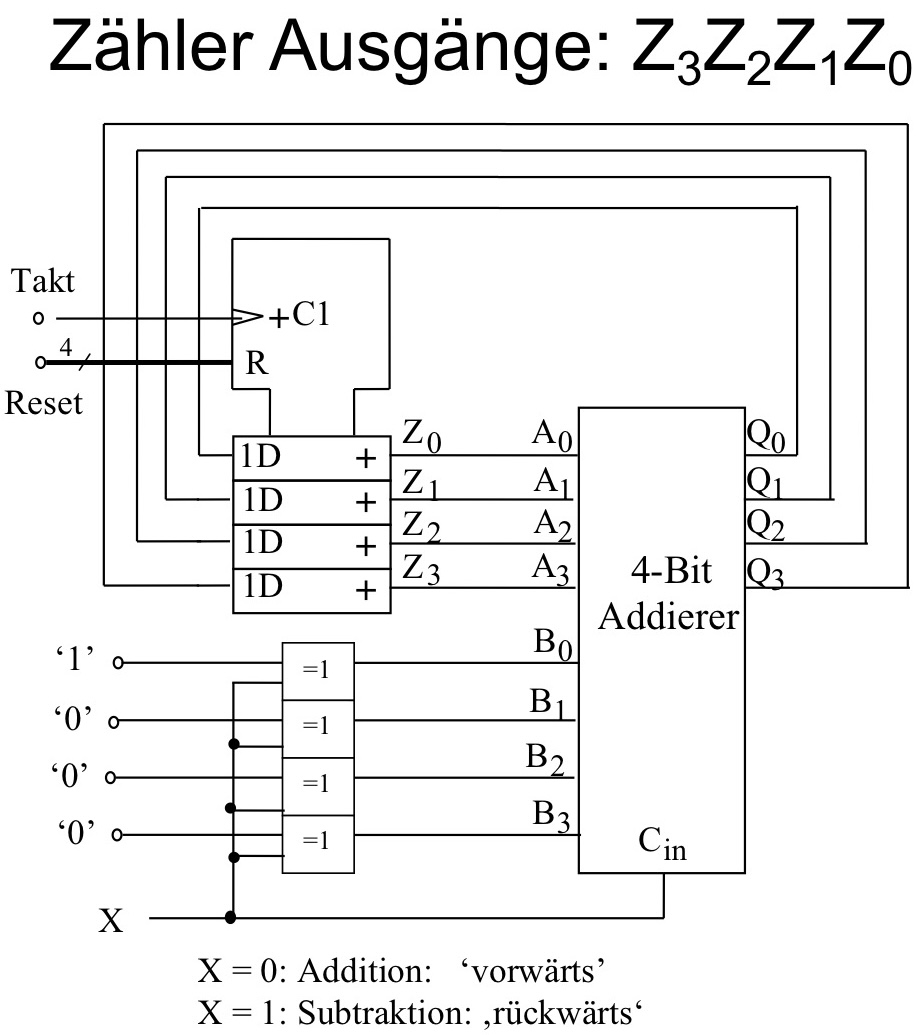
\includegraphics[width = 50mm]{images/forward_back_count.JPG}
\end{center}
D-FlipFlops mit Addierer kombinieren.
\begin{flushleft}
    \begin{tabular}{c c c c l}
        $X$ & $B_3 B_2 B_1 B_0$ & & & \\
        $0$ & $0001$ & $\rightarrow$ & $+1$ & \multirow{2}{*}{addiert}\\
        $1$ & $1111$ & $\rightarrow$ & $-1$ & 
    \end{tabular}
\end{flushleft}